

\subsection{ASCR Focus Areas}

There are many opportunities for return on investment in HPC correctness.  These returns and investments would fall into the short, medium and long term time scales.

\subsubsection{Short Term}

\paragraph{Advances for production use.}
Investment focused on supporting the current efforts to program and perform computational science on leadership computing facilities.  Such effort would apply best-of-breed existing tools (commercial as well as those being researched by the community), extend those tools, and generally work with HPC applications code as-is.  Such work would encompass extending the existing HPC tools infrastructure (debuggers, compilers, etc.) with features for larger scale verification and debugging in the more complex HPC contexts being encountered today.

% by ganesh
\begin{WrapText}
\footnotesize
 
 We propose many directions
 broken down into short, medium and
 long-term components.
 %
 We also propose
 an agenda for a correctness
 workshop as well as 
 a few   ``moonshot'' projects
 that can bring in added creativity through added time and resource pressures.
 
\end{WrapText}
\paragraph{Importing successful ideas from non-HPC domains.}
This effort would focus on bringing the tools and technologies currently being developed to prove correctness and safety properties of non-HPC code, to the HPC community.  This would bring software currently being used to formally prove hardware, security, safety, and performance---as applicable---to HPC.  Research in the formal verification of cyber-physical systems could be applied to the verification of simulated physical systems.  Research in embedded computing - e.g. verification of controls, and verified hardware, e.g. flight safety, could be applied to verifying the controls for current HPC systems.  Certification techniques for large scale distributed systems (e.g., Amazon, DropBox) could be brought to HPC for reasoning about large scale parallel computing systems (and HPC file systems).

\subsubsection{Medium Term}

\paragraph{Community-wide impact:} Medium term focus must target achieving community-wide impact  through projects that take on the challenges of 
verifying critical software components such as  widely-used runtime systems (e.g., OpenMP and MPI implementations) and math libraries.
%
There must also be significant emphasis placed on the collection of bug incidence reports, as well as search for past solutions that detail how these bugs were fixed.
%
Finally,  tool interfaces and runtime event collection mechanisms must be standardized to support tool composition.

% by ilaguna
\begin{figure}
\label{figure:goals}
\centering
\begin{adjustbox}{width=1.15\textwidth,center}
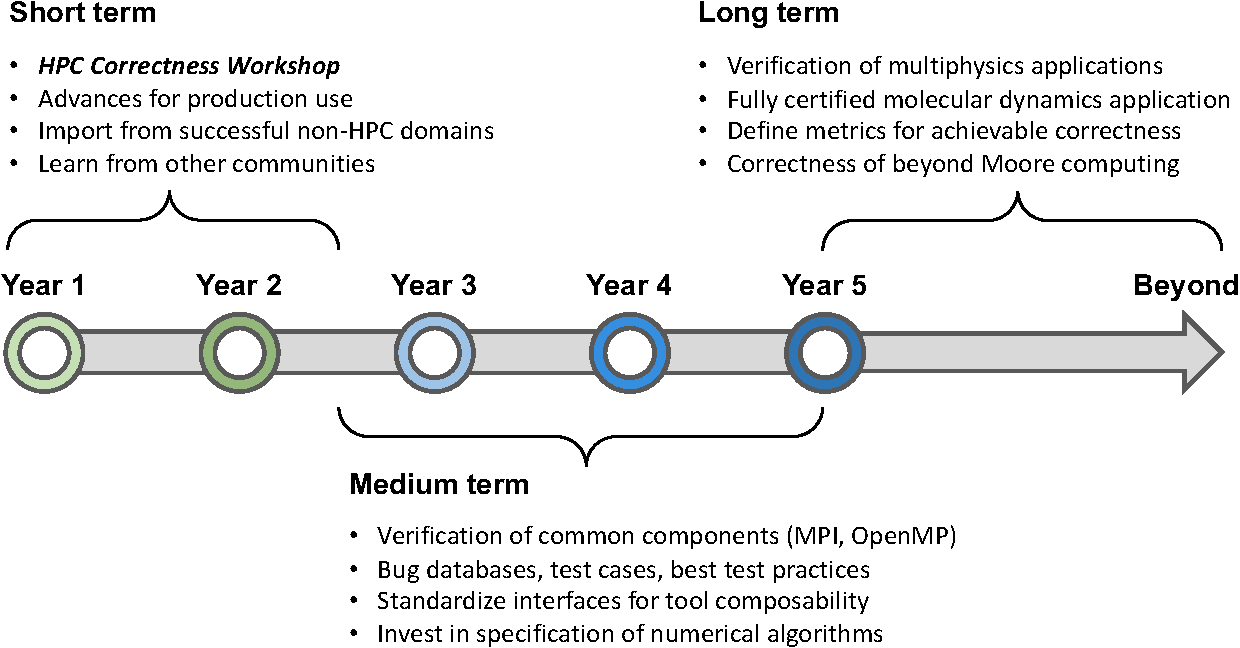
\includegraphics[width=0.99\textwidth]{figures/future_goals.pdf}
\end{adjustbox}
\caption{Short, medium, and long term goals identified to advance the field of correctness in HPC}
\end{figure}


\paragraph{Ontologies of mathematics / algorithms.}
This effort would focus on developing specific infrastructure for verification and debugging unique to HPC.  In particular, investments in the modeling and specification of numerical algorithms, ontologies for the mathematics underlying such algorithms, and reasoning about statistical and randomized systems, would be advanced.  There would likely be a close relationship between these efforts and Uncertainty Quantification and Automatic Differentiation, since such efforts are aimed at giving confidence in the results of scientific simulations.  Research would be aimed at tools for automated reasoning and verification about topics in Applied Mathematics of relevance to ASCR, in particular numerical methods for scalable solving of PDEs, discretization, optimization, multi-scale computing, and multi-physics. The effort would be directed toward formalizing mathematics otherwise expressed in ``prose'' in mathematical research papers.  The effort would try to parallel the development seen in the computer systems research community, where new systems software research papers (operating systems, file systems, etc.) are now expected to come with the formal expression of the algorithm and the proof of its correctness.  Such an effort would nudge and enable the engineering of these new mathematical advances to be done with the most modern software engineering practices, with the modularity, specifications, and proofs needed to achieve correct by construction HPC systems.  

\subsubsection{Long Term}
 
\paragraph{Beyond Moore.}
Focus on Beyond Moore computing would clearly be an appropriate  long term focus.  In particular, ensuring correctness of new computing paradigms such as neuromorphic, probabilistic, and quantum computation.  Application areas such as machine learning would also be a focus of the correctness research.  Machine learning in particular seems to offer opportunities for new advances in correctness, particularly developing systems for proving that a ML system will work within bounds, and for explaining the conclusions or decision made by a machine learning system.

\paragraph{``Moonshot'' projects.}
Longer term investments would be achieved by moonshot projects that seek to build end-to-end, demonstrable successes, with both immediate benefits and which also become the basis for advances in the field.
%We designate such projects IAFRE, for Integrated Ambitious Focused Research Efforts.
A few potential moonshot projects are described in \S\ref{sec:iafre}.

\subsection{Moonshots}
\label{sec:iafre}

Well-chosen ``moonshot'' challenges can help increase the pace of progress and demonstrate what is possible.  While these projects are ambitious, they are probably feasible with just a few years of focused effort.  Consider that the first sequencing of a human genome took about ten years and billions of dollars, but now such sequencing is routinely practiced within a few hours in a doctor's office lab for a few hundred dollars.  Once feasibility is established in the projects below, the engineering of tools to reduce costs and speed the results will rapidly advance.  For verification in particular, consider that proof libraries and tools are cumulative, and can lead to building of capabilities.  The first efforts to formalize floating point took years to achieve, but the formal specifications for floating point are now available and can 
be downloaded for free.

\subsubsection{Project 1: Fully certified molecular dynamics simulation}  

% has since 2006 provided full determinism and {\em bitwise time reversibility}, even as it uses the best models, optimizations and algorithms available for the highest performance simulation of molecular dynamics of any tool.  DESMOND demonstrates that the behavior of the MD algorithm is extremely well controlled and understood, when carefully coded.  A moonshot project would be to enhance DESMOND

% Other MD packages could the basis for this IAFRE, but they would first have to be modified to match DESMOND's bitwise time reversibility and performance. to provide a fully certified implementation, in the context of a formally specified and verified HPC hardware system.  

Molecular dynamics (MD) packages such as Desmond~\cite{bowers2006scalable} would serve as excellent ``moonshot'' projects.  The tools and science of projects such as Deep Specification~\cite{Pierce:SPLASHTalk2016} could be applied, extending them to the special tuned number representations and operators of DESMOND, through bond models and approximations, and through the compiler, systems software, and runtime.  One would certify the property of bit-reversibility through to the implementation.  The components of such a project (e.g., a fully certified concurrent dynamic runtime task scheduler, certified parallel 3D FFT) could then be used in other projects. 

Longer term, this technique could be used to provide certifications and verification that a long running numerical simulation running on a special purpose scientific computer {\em proves} a scientific result~\cite{sussman1992chaotic}.  This would not just be an academic exercise; vital missions of the Department of Energy (e.g., the NNSA) depend on simulation on complex, custom constructed high performance computers to assure the safety and performance of our nation's strategic nuclear arsenal. Advances in NNSA simulations of kinetic plasma on the special Roadrunner supercomputer~\cite{bowers2009advances} used optimizations and coding techniques closely relate to those of DESMOND.  The results of such moonshot projects could immediately carry over to kinetic plasma simulations of the type that runs on Roadrunner.  Furthermore, such a certification system could be used to assess the implications of new hardware architectures (e.g., network communications protocols), representations (reducing the precision of values) and algorithms (e.g., communication avoiding or sparse high dimensional FFT) on future high performance kinetic plasma simulations.

\subsubsection{Project 2: Multiphysics}
Multiphysics software systems---simulations that consists of more than
one component governed by its own principles---are used in many large-scale physical simulations.
%
An impactful project would be full verification of important logic and numerical properties (e.g., energy conservation properties or others) underlying multiphysics applications.
%
This exercise can force the examination of how individual subsystem guarantees help meet whole-system correctness goals.
%
Some examples of HPC multiphysics software infrastructures that could be targeted are Chombo~\cite{Chombo}, PETSc~\cite{PETSc}, SUNDIALS~\cite{SUNDIALS}, Trilinos~\cite{Trilinos}, and Uintah~\cite{Uintah}.

\subsubsection{Project 3: Verified Compiler/Runtime Components}
Verifying some of the key software infrastructural components of an HPC system can bootstrap the development of rigorous methods that help harden support for large-scale runs of HPC simulations.
%
Of special interest would be the verification of the MPI library, going by the MPI 4.0 standard, tracing through various device layers and ending in optimized infrastructural code that supports rapid messaging using lock-free programming methods.
%
Similarly, verifying the polyhedral compilation toolchain and linear algebra libraries can ensure correctness of large and highly reused code bases.


\subsection{HPC correctness workshop}
The exercise of bringing this limited set of report authors together for sharing ideas has resulted in good cross fertilization of ideas for HPC correctness: making us aware of useful tools for our own research in HPC, and some of the larger challenges.  But with the breadth of the problem, and the richness of the verification and debugging community outside, HPC, more is needed.

Advancement in this area of correctness could be facilitated by a workshop on HPC correctness that could bring together the larger community of experts on correctness techniques and tools with DOE stakeholders, especially the developers of DOE HPC applications. 

Such a workshop would provide an opportunity for HPC software developers to communicate current practices and discuss the primary obstacles to achieving correctness in HPC software development and for correctness experts to identify promising research directions that offer the potential to overcoming these obstacles.  A two day workshop comprising a small number of invited presentations, 5--10 minute presentations based on 2-page position papers solicited from the community, and 3--4 1-hour round table discussions to stimulate a dialogue between the correctness experts and stakeholders is recommended.  We anticipate that this dialogue will reinforce many of the summit findings, possibly identify additional research opportunities, and help prioritize future research directions.
%--


\subsection{Competitions for verification of HPC software}

In recent years, several verification competitions have evolved within the general software verification community.
For example, the annual SV-COMP competition, currently in its seventh year~\cite{sv-comp}, is a fully automated competition in which participants submit tools which are all fed a long series of C programs with corresponding properties that are expected to hold or fail.  The VerifyThis competition~\cite{verify-this}, in its sixth year, is an interactive competition in which participants are given a set of problems which they are expected to implement and verify over the course of a day using any tools they desire.
These competitions have had several beneficial impacts: they provide objective and consistent comparisons of tools, they provide a recognized measure of the current state-of-the-art, and they have created large verification benchmark suites that are widely used beyond the competition itself.

As discussed above, HPC software has many specific characteristics, and these are not covered in the existing general-purpose software competitions.  Therefore, a HPC-specific verification competition could be held, say, during the course of one day at SC17 with multi-agency sponsorship.   Similar to VerifyThis, participants could be given a set of programs of increasing complexity, together with written specifications of expected behavior, and asked to formally specify and verify as much as they can, using any tools they desire.   A panel of judges would examine and evaluate the results.  Participants could also be given an opportunity to present their solutions.

